\documentclass{proc}

\title{Exploring Neural Networks optimisations with an application in handwriting recognition engines}
\author{Stefanos Stefanou(020363)}
\usepackage[margin=0.3in]{geometry}
\usepackage{amsmath}
\usepackage{tikz}
\usepackage{textgreek}
\usepackage{listings}
\usetikzlibrary{positioning}
\usepackage{array}
\usepackage{multirow}
\usepackage{url}
\usepackage{graphicx}
\newcommand\MyBox[2]{
	\fbox{\lower0.75cm
		\vbox to 1.7cm{\vfil
			\hbox to 1.7cm{\hfil\parbox{1.4cm}{#1\\#2}\hfil}
			\vfil}%
	}%
}
\tikzset{%
	every neuron/.style={
		circle,
		draw,
		minimum size=0.1cm
	},
	neuron missing/.style={
		draw=none, 
		scale=1,
		text height=0.1cm,
		execute at begin node=\color{black}$\vdots$
	},
}
\begin{document}
	\maketitle
	\section{Abstract}
	Multilayer Neural Networks trained using back-propagation algorithm are the best example of a successful
	Gradient-Based learning technique. In this report, we will be going to explore an application of an MN N, handwritten pattern recognition. We will tune our MN N application to be able to handle efficiently the dozens of thousands of samples of MNIST Databases, using basic linear algebra rules.
	\section{Introduction}
	\subsection{Structure}
	We have used a minimal yet powerful OOP approach to synthesize our solution, with 2 basic classes, NeuralNetwork and PerceptronMultilayer. NeuralNetwork class is a wrapper over multiple PerceptronMultilayer objects.it handles and supervises their learning by injecting them the proper data during learning.
	\subsection{The Algorithm}
	To perform our experiments in a reasonable amount of time, a new approach was needed. so we we-wrote our Multilayer Neural Network engine, using matrix multiplications. this reduced the learning time significantly.
	\subsubsection{Calculating a layer}
	let the following sigmoid-activated MNN.
	
	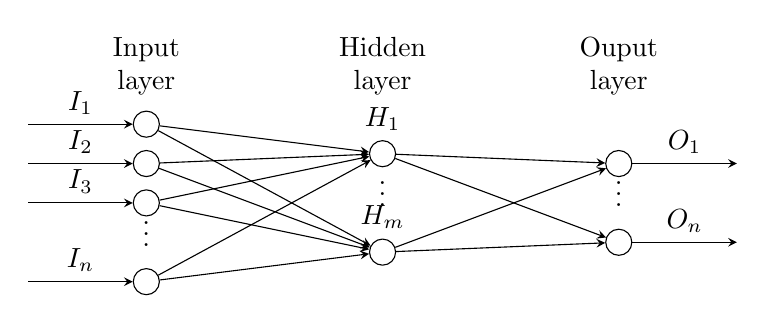
\begin{tikzpicture}[x=1.5cm, y=0.5cm, >=stealth]
	
	\foreach \m/\l [count=\y] in {1,2,3,missing,4}
	\node [every neuron/.try, neuron \m/.try] (input-\m) at (0,2.5-\y) {};
	
	\foreach \m [count=\y] in {1,missing,2}
	\node [every neuron/.try, neuron \m/.try ] (hidden-\m) at (2,2-\y*1.25) {};
	
	\foreach \m [count=\y] in {1,missing,2}
	\node [every neuron/.try, neuron \m/.try ] (output-\m) at (4,1.5-\y) {};
	
	\foreach \l [count=\i] in {1,2,3,n}
	\draw [<-] (input-\i) -- ++(-1,0)
	node [above, midway] {$I_\l$};
	
	\foreach \l [count=\i] in {1,m}
	\node [above] at (hidden-\i.north) {$H_\l$};
	
	\foreach \l [count=\i] in {1,n}
	\draw [->] (output-\i) -- ++(1,0)
	node [above, midway] {$O_\l$};
	
	\foreach \i in {1,...,4}
	\foreach \j in {1,...,2}
	\draw [->] (input-\i) -- (hidden-\j);
	
	\foreach \i in {1,...,2}
	\foreach \j in {1,...,2}
	\draw [->] (hidden-\i) -- (output-\j);
	
	\foreach \l [count=\x from 0] in {Input, Hidden, Ouput}
	\node [align=center, above] at (\x*2,2) {\l \\ layer};
	
	\end{tikzpicture}
	The calculation of a single layer can be done by multiplying the weights of the current layer with the transposed matrix inputs.
	
	\[
	\begin{bmatrix}
	w_{11} & w_{12} & w_{13} & \dots  & w_{1m} \\
	w_{21} & w_{22} & w_{23} & \dots  & w_{2m} \\
	\vdots & \vdots & \vdots & \ddots & \vdots \\
	w_{m1} & w_{m2} & w_{m3} & \dots  & w_{nm}
	\end{bmatrix}
	\begin{bmatrix}
	x_{1}\\
	x_{2}\\
	\vdots\\
	x_{m}
	\end{bmatrix}
	=
	\begin{bmatrix}
	$$\sum_{i=1}^{n} x_iw_{1i}$$ \\
	$$\sum_{i=1}^{n} x_iw_{2i}$$ \\
	\vdots \\
	$$\sum_{i=1}^{n} x_iw_{mi}$$
	\end{bmatrix}
	\]

	The following python code implements this algorithm.
	
		\begin{lstlisting}[language=Python]
def run(self, prev_layer_out):
  sum=np.dot(self.weights,prev_layer_out.T)
  result=sigmoid(sum)
  return result.T
	\end{lstlisting}
	 \subsubsection{Training the output layer}
	 Let the $M$ targets, $O$ be the outputs(after the activation function is applied) and $I$ be the inputs of the output layer.
	 \[
	 T=
	 \begin{bmatrix}
	 t_{1}\\
	 t_{2}\\
	 \vdots\\
	 t_{m}
	 \end{bmatrix}, 	 
	 O=
	 \begin{bmatrix}
	 o_{1}\\
	 o_{2}\\
	 \vdots\\
	 o_{m}
	 \end{bmatrix},
	 I=
	 \begin{bmatrix}
	 i_{1}\\
	 i_{2}\\
	 \vdots\\
	 \vdots\\
	 i_{n}
	 \end{bmatrix}    
	 \]
	 Then, by defining ${\odot}$ to be Hadamard multiplication, the matrix of deltas in the output layer will be.
	 \[
	 \Delta=
	 (T-O)\odot(1-O)\odot O=
	 \begin{bmatrix}
	 (t_{1} - o_{1})(1-o_{1})o_{1}\\
	 (t_{2} - o_{2})(1-o_{2})o_{2}\\
	  \vdots\\
	 (t_{m} - o_{m})(1-o_{m})o_{m}
	  \end{bmatrix} 
	 =
	 \begin{bmatrix}
	 \delta_1\\
	 \delta_2\\
	 \vdots\\
	 \delta_m
	 \end{bmatrix} 
	 \]
	Let \texteta{} be the MNN's learning rate, then the correction matrix will be
	\[
	C=I(\Delta\eta)^T= 
	\begin{bmatrix}
		\delta_1i_1\eta & \delta_1i_2\eta & \delta_1i_3\eta & \dots  & \delta_1i_m\eta \\
		\delta_2i_1\eta & \delta_2i_2\eta & \delta_2i_3\eta & \dots  &  \delta_2i_m\eta \\
		\vdots & \vdots & \vdots & \ddots & \vdots \\
		\delta_ni_1\eta & \delta_ni_2\eta & \delta_ni_3\eta & \dots  & \delta_ni_m\eta
	\end{bmatrix}
	\]
	The python code, implementing this algorithm, is given below
	\begin{lstlisting}[language=Python]
def term_learn(self, i, o, t):
  t=t.reshape(1,self.output_len)
  o=t.reshape(1, self.output_len)
  Delta=np.array((t-o)*(1.0-o)*o)
  correction=i*Delta.T
  self.weights+=correction
	\end{lstlisting}
	\subsubsection{Training the hidden layer}
	Let the $\Delta_r$, W\textsubscript{r} be the deltas and the weight matrices  of r'th layer respectively
	\[
	\Delta_r=
	\begin{bmatrix}
	\delta_1\\
	\delta_2\\
	\vdots\\
	\delta_n
	\end{bmatrix} 	 
	W_r=
	\begin{bmatrix}
	w_{11} & w_{12} & w_{13} & \dots  & w_{1m} \\
	w_{21} & w_{22} & w_{23} & \dots  & w_{2m} \\
	\vdots & \vdots & \vdots & \ddots & \vdots \\
	w_{n1} & w_{n2} & w_{n3} & \dots  & w_{nm}
	\end{bmatrix} 
	\]
	Next, we define ${E_r(i)}$ to be the error of i'th neuron at r'th layer
	\[ E_r(i)=\sum_{j=1}^{n} \delta_{r+1}(j)*w_{r+1}(j,i)  \]
	It can be easily seen that the following statement is true
	\[
	W_{r+1}^T\Delta_{r+1}=
	\begin{bmatrix}
	\sum_{j=1}^{n} \delta_{r+1}(j)*w_{r+1}(j,1)\\
	\sum_{j=1}^{n} \delta_{r+1}(j)*w_{r+1}(j,2)\\
	\vdots\\
	\sum_{j=1}^{n} \delta_{r+1}(j)*w_{r+1}(j,m)
	\end{bmatrix} 
	=
	\begin{bmatrix}
	 E_r(1)\\
	 E_r(2)\\
	\vdots\\
	 E_r(m)
	\end{bmatrix} 
	\]
	
	So ,our delta matrix will become
	\[
	\Delta_r=
	W_{r+1}^T\Delta_{r+1}\odot(1-O)\odot O=
	\begin{bmatrix}
	E_r(1)(1-o_{1})o_{1}\\
	E_r(2)(1-o_{2})o_{2}\\
	\vdots\\
	E_r(m)(1-o_{m})o_{m}
	\end{bmatrix} 
	=
	\begin{bmatrix}
	\delta_1\\
	\delta_2\\
	\vdots\\
	\delta_m
	\end{bmatrix} 
	\]
	The rest of the procedure is identical to section 2.2.2. The following code implements this algorithm.
	\begin{lstlisting}[language=Python]
def mid_learn(self,i,next_layer,o):
  Wr_p_1=next_layer.weights
  Dr_p_1=next_layer.Delta
  self.Delta=Wr_p_1.T*Dr_p_1
  self.Delta=self.Delta*(1-o)*o
  self.Delta=i*self.Delta.T*self.learning_rate
  self.weights+=self.Delta
	\end{lstlisting}
	\subsection{Technologies}
	In our application, we have used several new technologies to cope with the natural complexity of the given task. We completely rewrote our Multilayer Neural Network engine using python3.6, to have available the following tools available, as a result.
	\subsubsection{numpy}
	NumPy is a mathematics library for python. It offers fast matrix multiplication and dot product implementations, vital for our approach in MN N's
	\subsubsection{matplotlib}
	Matplotlib is a plotting library for python, we used to visualize our data and results
	\subsubsection{pickle}
	Pickle is a python object serializer module, it offers fast de-serialization which is vital for our time-sensitive application.	
	\section{User Application}
	The MNIST Database(Modified National Institute of Standards and Technology)consists of 60.000 train and 10.000 test examples of handwritten digits. It is a standardized test in machine learning and is used as a common ground for researches to compare their results.
	
	Our dataset is contained in 2 CSV files in which our training and testing data are included. Every line of these files consists of a 28x28 image, given as exactly 784 numbers, between 0(white pixel) and 255(black pixel). An additional number at the beginning of each line is for the numbers label.
	\subsection{Preprocessing}
	\subsubsection{Normalised Labels}
	As our task involves classification, we need to convert our numerical labels to categorical ones, so we need to perform "Binarization" to MNIST's labels. We will use the one-hot representation. Each line of every CSV file starts with a number ${k[0<=k<=9]}$ witch will be converted in a 9x1 matrix as follows
	
	\begin{center}
		\begin{tabular}{ |c|c| } 
			\hline
			Numerical labels & Categorical labels \\
			\hline
			 0 & [1000000000] \\ 
			 1 & [0100000000] \\ 
			 \dots & \dots \\
			 8 & [0000000010] \\ 
			 9 & [0000000001] \\ 
			\hline
		\end{tabular}
	\end{center}
	\subsubsection{Normalised Pixels}
	We will convert the default grayscale interval to a range [0,1], by dividing each pixel value with 255. At a first glance, this seems a nice solution for converting our data suitable for our MNN, but our experimentation revealed a fatal flaw, This technique allows, zero inputs, something that if occur can prevent the neuron from learning. We can solve this issue by applying the following transformation to every pixel.
	\[
		f(x)=\frac{x*0.99}{255}+0.01
	\]
	\subsection{Initialization}
	Initialization is a very important factor in our application success, we cant choose arbitrary initialization weights. Weight matrices should be chosen randomly but not arbitrary[2]. By choosing a random normal distribution as our weight generator, we have broken possible symmetries, which may affect negatively the learning process[2].
	
	Let ${n}$ be the number of inputs in our network, our initialization procedure draws random numbers from a $truncated$ normal distribution as follows
	
	\[
		{\displaystyle X\sim{\frac {1}{\sigma }}\,{\frac {\phi ({\frac {x-\mu }{\sigma }})}{\Phi ({\frac {b-\mu }{\sigma }})-\Phi ({\frac {a-\mu }{\sigma }})}}},
		\mu=0,
		\sigma=1
	\]
	with the following, commonly used bounds (Glorot, Xavier and Bengio, Y, 2010)
	\[	a=-\frac{1}{\sqrt(n)},
		b=\frac{1}{\sqrt(n)},
	\] 
	\subsection{Fragmentation of data}
	MNIST Database has already provided us with a basic fragmentation of our data. 60.000 train and 10.000 test elements, but extensive care have been given in order to minimize the uncertainty factor and not over-train our MNN[1].
	
	the fraction of patterns reserved for the
	validation set should be inversely proportional to the square root of the number of free adjustable
	parameters.[1]
	
	The following table shows our data fragmentation scheme
	\begin{center}
		\begin{tabular}{ |c|c| } 
			\hline
			Category & Number of data\\
			\hline
			Train & 60000 \\ 
			Test & 6000 \\ 
			Validation & 4000 \\ 
			\hline
		\end{tabular}
	\end{center}

	\subsection{Structure of MNN}
	In order to ensure the optimal output, multiple experiments will be performed, using various Neuron and hidden layers configurations. As a common ground though, the following rules will be followed in every experiment.
	
	\begin{itemize}
		\item Every pixel will become a free adjustable parameter, in the input layer. So its expected that the input layer will always consist of 784 nodes
		\item As handwritten digits is a purely categorical variable, the output layer will always consists of 10 Neurons, one for each category(please refer to section 3.1.1)
	\end{itemize}
	
	 
	\begin{tikzpicture}[x=1.5cm, y=0.5cm, >=stealth]
	
	\foreach \m/\l [count=\y] in {1,2,3,missing,n}
	\node [every neuron/.try, neuron \m/.try] (input-\m) at (0,2.5-\y) {};
	
	\foreach \m [count=\y] in {1,missing,2}
	\node [every neuron/.try, neuron \m/.try ] (hidden-\m) at (2,2-\y*1.25) {};
	
	\foreach \m [count=\y] in {1,missing,2}
	\node [every neuron/.try, neuron \m/.try ] (output-\m) at (4,1.5-\y) {};
	
	\foreach \l [count=\i] in {1,2,3,\textsuperscript{784}}
	\draw [<-] (input-\i) -- ++(-1,0)
	node [above, midway] {$I_\l$};
	
	\foreach \l [count=\i] in {1,m}
	\node [above] at (hidden-\i.north) {$H_\l$};
	
	\foreach \l [count=\i] in {1,\textsuperscript{10}}
	\draw [->] (output-\i) -- ++(1,0)
	node [above, midway] {$O_\l$};
	
	\foreach \i in {1,...,4}
	\foreach \j in {1,...,2}
	\draw [->] (input-\i) -- (hidden-\j);
	
	\foreach \i in {1,...,2}
	\foreach \j in {1,...,2}
	\draw [->] (hidden-\i) -- (output-\j);
	
	\foreach \l [count=\x from 0] in {Input, Hidden, Ouput}
	\node [align=center, above] at (\x*2,2) {\l \\ layer};
	
	\end{tikzpicture}
	\section{Results}
	\subsection{Accuracy criteria}
	There are plenty of metrics for machine learning algorithms evaluation, we choose to evaluate our solution using the Test Error Rate. This choice will enable us to compare our results directly with other researchers(please refer to section 5)
	
	let the following confusion matrix
	
	\noindent
	\renewcommand\arraystretch{1.5}
	\setlength\tabcolsep{0pt}
	\begin{tabular}{c >{\bfseries}r @{\hspace{0.7em}}c @{\hspace{0.4em}}c @{\hspace{0.7em}}l}
		\multirow{10}{*}{\parbox{1.1cm}{\bfseries\raggedleft actual\\ value}} & 
		& \multicolumn{2}{c}{\bfseries Prediction outcome} & \\
		& & \bfseries p & \bfseries n & \bfseries total \\
		& p$'$ & \MyBox{True}{Positive} & \MyBox{False}{Negative} & P$'$ \\[2.4em]
		& n$'$ & \MyBox{False}{Positive} & \MyBox{True}{Negative} & N$'$ \\
		& total & P & N &
	\end{tabular}

	We define accuracy $A$ as
	\[
		A={\frac {TP+TN}{FN+FP+TP+TN}}
	\]
	Test error $E$ is defined, as the complementary of Accuracy
	\[
		E = 1-A
	\]
	\subsection{Experiment setup}
	In order to avoid over-fitting, we apply a number of strategies. As Mark Twain once said, 'We should be careful to get out of an experience only the wisdom that is in it-and stop there'(From Following the Equator, 1897.)[4]
	\subsubsection{Number of Neurons}
	There is a common yet simple heuristic[4] for finding the maximum amount of neurons ${N_h}$ for a problem, without over-fitting a model
	\[
		N_h = \frac{N_s} {(\alpha * (N_i + N_o))}	
	\]
	\begin{itemize}
		\item $N_i$ = Number of input neurons
		\item $N_o$	= Number of output neurons
		\item $N_s$ = Number of samples in training data set
		\item $\alpha$ =   Model Generalisation Constant ${2<=\alpha<=10}$
	\end{itemize} 
	\subsubsection{Number of hidden layers}
	Additionally,1 hidden layer will suffice in our classification application. It is easily shown[4] that 
	
	\begin{itemize}
		\item 0 Hidden layers can learn only linear separable functions
		\item 1 Hidden layers can approximate any function that contains a continuous mapping from one finite space to another
		\item 2 Hidden layers can approximate any smooth mapping to any accuracy(dangerous for overfitting in our classification problem)
	\end{itemize} 
	
	An additional experiment with 2 hidden layers will be performed at the end, but with high generalisation constant, to avoid over-fitting our model.
	
	\subsection{1 hidden layer Performance}
	In the following graph, the average error rates of 50 runs are presented for various Generalization constants.
	\begin{figure}[!h]
		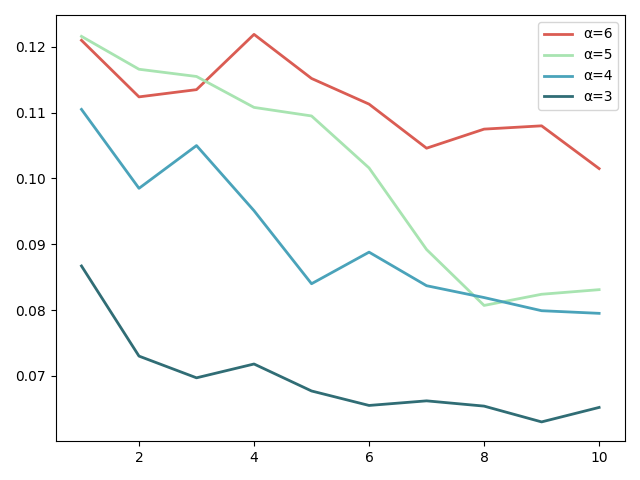
\includegraphics[width=\linewidth]{genone.png}
		\caption{Average T Error vs Epochs vs $\alpha$}
		\label{fig:1-X-1}
	\end{figure}

	As we are in 1 hidden layer, the probability of over-fitting is relatively small compared with 2 or more hidden layer configurations, so we choose our Generalisation constant $\alpha \in [3,6]$
	
	There is a clear and expected trade-off, as the model tends to generalise, the error rate rises significantly.
	However it becomes evident that we can get a accurate enough classifier $(\sim 10\% $ T-Error) even with the most conservative settings(${a=4  || a=5}$)
	\subsection{2 hidden layers Performance}
	As we are in 2 hidden layer now, the probability of over-fitting is higher compared with 1 hidden layer configuration, so we choose a higher Generalisation constant  $\alpha \in [5,8]$
	
	In the following graph, the average error rates of 50 runs are presented for various Generalization constants within our predetermined range. Our setup uses the same amount of neurons in both hidden layers
	
	\begin{figure}[!h]
		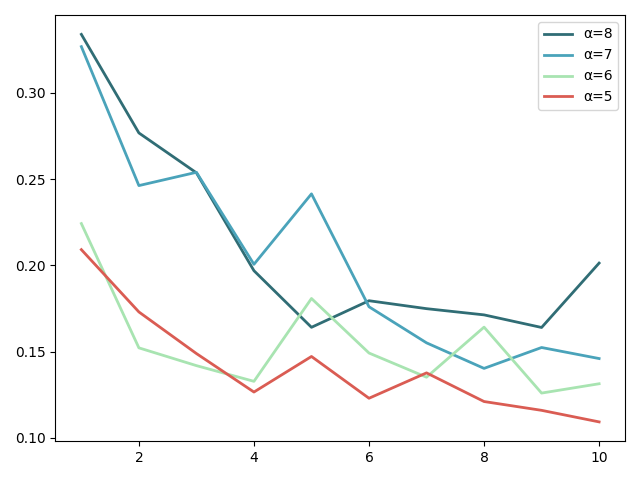
\includegraphics[width=\linewidth]{gentwo.png}
		\caption{Average T Error vs Epochs vs $\alpha$}
		\label{fig:1-X-1}
	\end{figure}
	
	It becomes evident that we can get a accurate enough 2 hidden layer classifier $(\sim 15\% $ T-Error) even with the most conservative settings(${a=6  || a=7}$)
	

	\section{Comparison}
	
	After experimentation, based on our target to find the most accurate yet generalised model, we narrowed down our results to the following classifiers.
	
	\begin{center}
		\begin{tabular}{ |c|c|c| }
			\hline
			Network Type&Generalization constant &Average Error Rate \\
			\hline
			1 Hidden &4  & 0.090 \\
			1 Hidden &5  & 0.101 \\
			2 Hidden &6  & 0.15 \\
			2 Hidden &7  & 0.20 \\
			\hline
		\end{tabular}
	\end{center}

	MNIST Database contains a table with various research publications relating the MNIST task. Under the linear classifiers section, our results for 1-Hidden MNN are closely related with publication[5]
	
	\begin{center}
		\begin{tabular}{ |c|c|c| }
			\hline
			Origin&Network Type&Average Error Rate \\
			\hline
			Our results&1 Hidden& 9\% \\
			Our results&1 Hidden& 10\% \\
			LeCun et al.[5]&1 Hidden  & 12\% \\
			LeCun et al.[5]&1 Hidden  & 8\% \\
			\hline
		\end{tabular}
	\end{center}
 
	Our results for 2-Hidden MNN's are significantly lower with publication [5]
	\begin{center}
		\begin{tabular}{ |c|c|c| }
			\hline
			Origin&Network Type&Average Error Rate \\
			\hline
			Our results&2 Hidden& 15\% \\
			Our results&2 Hidden& 20\% \\
			LeCun et al.[5]&2 Hidden  & 5\% \\
			LeCun et al.[5]&2 Hidden  & 4\% \\
			\hline
		\end{tabular}
	\end{center}

	This is something to be expected though, because our goal is to create a generalised model, under this circumstances, some compromises in performance need to be made
	
	\section{Discussion}
	Our end goal is to create a tool for recognising hand written patterns, and possibly in the future(side/personal project) to generalise this solution to a full hand written recognition engine. We are taking extensive care of not over-fit our model, something that will prove catastrophic for our application. With this limitations in mind, as our first simplistic attempt, a few performance compromises needed to be made to ensure our models safety. Even with the most conservative settings though, our first results were interesting enough. We are making optimistic predictions that an updated version of this engine using convolutional neural networks will be able to exceed 98\% accuracy in the near future
	\section{Conclusion}
	At this stage our solution is capable for recognising isolated hand written digits with a maximum accuracy(within safety limits) of 92\%. It becomes evident that there is a lot of work to do to generalise successfully this solution, mainly due to segmentation problems(where a digit start and where ends?) but we are remaining optimistic about the near future.
	\begin{thebibliography}{9}
		\bibitem{isab1} 
		Amari, Shun-ichi and Murata, Noboru and Müller, Klaus-Robert and Finke, Michael and Yang, Howard 
		\textit{Asymptotic Statistical Theory of Overtraining and Cross-Validation}. 
		IEEE transactions on neural networks 1997.
		
		\bibitem{knuthwebsite} 
		Bernd K: Neural Network Using Python and Numpy,
		\\\texttt{https://www.python-course.eu}
		
		\bibitem{init} 
		Glorot, Xavier and Bengio, Y. 
		\textit{Understanding the difficulty of training deep feedforward neural networks}. 
		Journal of Machine Learning Research - Proceedings Track 2010.
		
		\bibitem{nnbook} 
		Hagan, M-T. Demuth,H. Beale, Hudson M. De Jesús, O
		\textit{Neural Network Design}.
		1996
		
		\bibitem{result1} 
		Y. Lecun, L. Bottou, Y. Bengio and P. Haffner
		\textit{Gradient-based learning applied to document recognition}.
		in Proceedings of the IEEE. Nov. 1998.
		
	\end{thebibliography}

	\end{document}